\documentclass{jreport}
\usepackage{amsmath,amsthm,amssymb}
\usepackage{thmtools}
\usepackage[dvipdfmx]{graphicx}
\usepackage{float}
\usepackage{subfig}
\usepackage{caption}
\usepackage{color}
\usepackage{geometry}
\usepackage{algorithm,algpseudocode}
\usepackage{minted}
\usepackage{multicol}
\usepackage{enumerate}
\usepackage{verbatim}
\usepackage{mytitle}


\renewcommand{\thesubsection}{(\alph{subsection})}

\graphicspath{{../res/figure/}{../res/plot-the/}}
\makeatletter
\def\input@path{{../res/figure/}{../res/graph/}{../res/table-the/}}
\makeatother

% define command for pandoc
\providecommand{\tightlist}{\setlength{\itemsep}{0pt}\setlength{\parskip}{0pt}}

% setting margin
\newgeometry{tmargin=2cm,lmargin=2cm,rmargin=2cm,bmargin=2cm}

% adding new symbol (vrectangle and vrectangleblack)
\DeclareFontEncoding{LS1}{}{}
\DeclareFontSubstitution{LS1}{stix}{m}{n}
\DeclareSymbolFont{symbolsstix}{LS1}{stixscr}{m}{n}
\DeclareMathSymbol{\vrectangleblack}{\mathord}{symbolsstix}{"C5}
\DeclareMathSymbol{\vrectangle}{\mathord}{symbolsstix}{"C6}

% add math operator
\DeclareMathOperator*{\argmin}{\arg\!\min}
\DeclareMathOperator*{\argmax}{\arg\!\max}

% theorem preference
\declaretheoremstyle[
  spaceabove=1ex, 
  numbered=yes,
  headfont=\bfseries,
  headpunct=,
  bodyfont=\normalfont,
  spacebelow=1ex,
]{mythmstyle}
\declaretheorem[
  parent=chapter,style=mythmstyle,qed=$\vrectangle$,title=定義,
]{definition}
\declaretheorem[
  style=mythmstyle,sibling=definition,qed=$\vrectangle$,title=例,
]{example}
\declaretheorem[
  style=mythmstyle,sibling=definition,title=補題,
]{lemma}
\declaretheorem[
  style=mythmstyle,sibling=definition,qed=$\vrectangle$,title=補題,
]{lemma-without-proof}
\declaretheorem[
  style=mythmstyle,sibling=definition,title=定理,
]{theorem}
\declaretheorem[
  style=mythmstyle,sibling=definition,qed=$\vrectangle$,title=定理,
]{theorem-without-proof}
\declaretheorem[
  style=mythmstyle,sibling=definition,title=系,
]{corollary}
\declaretheorem[
  style=mythmstyle,sibling=definition,qed=$\vrectangle$,title=系,
]{corollary-without-proof}
\declaretheorem[
  style=mythmstyle,sibling=definition,qed=$\vrectangle$,title=予想,
]{conjecture}
\renewcommand{\proofname}{\normalfont{[\,証明\,]}\nopunct}
\renewcommand{\qedsymbol}{$\vrectangleblack$}

% algorithm preference
\renewcommand{\listalgorithmname}{アルゴリズムリスト}
\renewcommand{\thealgorithm}{\arabic{chapter}.\arabic{algorithm}}
\makeatletter
\renewcommand{\ALG@name}{アルゴリズム}
\@addtoreset{algorithm}{chapter}
\makeatother

% minted preference
\usemintedstyle{friendly}

% bibtex preference
\renewcommand{\bibname}{参考文献}
\bibliographystyle{junsrt}


\title{一般化ムーアグラフの探索の\\高効率化と高速化}
\author{里谷 佳紀}
\date{\today}
%\reportname{特 別 研 究 報 告 書}
\reportname{卒業論文}
\department{岡山大学工学部情報系学科}
\supervisor{高橋 規一}

\begin{document}

\maketitle


近年の急速なWebアプリケーションの発展に伴い,データセンタや大規模グラフ分析が
注目されている.これらの技術はスイッチの相互接続による計算機ネットワークが必要
である.ネットワークの性能はトポロジ(接続構造)によって変化する.
トポロジについて議論する際,ネットワークを正則グラフとして表現することが多い.
低遅延なネットワークを実現するグラフは,平均頂点間距離の値が小さいグラフで,
そのために平均頂点間距離が小さなグラフの構築が重要である.

平均頂点間距離が理論的な下界と一致する正則グラフは一般化ムーアグラフと呼ばれる.
現在まで,そのようなグラフを構築する方法がいくつか提案されてきた.しかし,
すべての頂点数と次数の組に対応することと,一般化ムーアグラフの性質を利用して
効率的に構築することの両方を満たす構築方法はまだ提案されていない.

そこで,本研究は,任意の頂点数と次数の組に対応し,その性質を利用して
効率的に一般化ムーアグラフを構築する方法を提案し,その有効性を実験で検証する
ことを目的とする.方法を詳細に説明すると,全探索を基本として,初期状態の変更や
枝刈りによって探索を高効率に行うものである.

実験の結果,頂点数と次数がそれぞれ$16$と$4$程度の場合,
全域木から探索を開始することと,直径の下界を用いた枝刈りが有効であることが
確認できた.


\tableofcontents

\chapter{序論}
近年,Webアプリケーションの発展により,ユーザの活動によって生み出される膨大な
データの収集と活用が大いに注目されている.それを実現する技術の一つに
データセンタが挙げられる.データセンタにはサーバが多数存在し,それぞれの
サーバがスイッチと接続し,さらにスイッチが相互に接続してネットワークを形成している
\cite{Greenberg2009,Al-Fares2008}.
ネットワークの性能はトポロジ(スイッチの接続構造)によって
変化するため,適切なトポロジを選択する必要がある.
最近,データセンタのネットワークにランダムトポロジを利用することが提案されている
\cite{Singla2011,Koibuchi2012}.このトポロジは,Fat-Tree\cite{Al-Fares2008}
などの従来のトポロジと比べてスケーラビリティで優れているなどの特徴がある
\cite{Singla2011}.

低遅延性はデータセンタのスループットに直結する重要な性質である.
したがって,低遅延を実現するネットワークの構築が重要である.
スイッチを頂点とみなしてネットワークを無向正則グラフでモデル化すると,
遅延は平均頂点間距離と密接に関連する.現在まで,
平均頂点間距離が小さいグラフの構築に関する研究が行われてきた.
例えば,2015年に藤田らは,辺の入れ替えを繰り返しながら
グラフの平均頂点間距離を小さくする方法を開発した\cite{Fujita2015}.
しかし,この方法では局所解に陥ることが多く,平均頂点間距離が最小である
グラフを発見することが困難である.

一方で,1973年にCerfらは,平均頂点間距離が小さい正則グラフとして一般化ムーアグラフを
提案し\cite{Cerf1973},翌年に一般化ムーアグラフの平均頂点間距離は
同じ頂点数と次数の正則グラフの中で下界であることを証明した\cite{Cerf1974Lower}.
一般化ムーアグラフを求める方法はいくつか知られている.
例えば,
2016年に山本らは正則グラフを列挙する佐藤らの方法\cite{Sato2008}を応用し,
一般化ムーアグラフが発見されるまで列挙を続ける方法を開発した
\cite{Yamamoto2016}.
しかし,この方法は,一般化ムーアグラフがもつ性質を利用して効率的に探索できて
いるとは言えない.

本研究では,与えられた頂点数と次数をもつ一般化ムーアグラフの
効率的探索法を提案し,その有効性を検証する.
まず,一般化ムーアグラフの基本的性質を説明し,
それに続いて,深さ優先探索に基づく探索アルゴリズムを与える.
その後,探索の初期状態の制限と枝刈りの導入によって探索空間を削減する手法を提案し,
それによって探索が効率化されることを実験的に示す.

%
\chapter{準備}
\label{chap:preliminary}
本章では,後の章に向けての準備をする.はじめに,グラフ理論の基本事項を説明する.
・・・などを含む.次に,Cerfらが提唱した一般化ムーアグラフの定義を与え,
いくつかの性質を証明する.これらの性質は,一般化ムーアグラフを探索する方法に
用いるもので,極めて重要である.

\section{グラフ理論の基本事項}
\label{sect:basic-graph-theory}
グラフ理論の基本事項を,\cite{Diestel2000}に則り説明する.
グラフ理論の基礎を理解している読者は\ref{sect:generalized-moore-graph}節まで
読み飛ばしても差し支えない.

\section{一般化ムーアグラフ}
\label{sect:generalized-moore-graph}
本節では一般化ムーアグラフを定義する.
さらに,これが満たすいくつかの性質を示す.

\begin{definition}[Cerf et.al., 1973\,\cite{cerf1973computer}]
  \label{def:generalized-moore-graph}
  次の性質が成り立つ頂点数$n$,次数$k$の正則グラフを
  \textbf{一般化ムーアグラフ}(\textbf{Generalized Moore graph})とよぶ.

  すべての頂点$v$について,$v$から$i$離れた頂点の数
  $c_i = \lvert\{ w\,|\,d(v,w) = i , w\in V \}\rvert$について,
  \[ \begin{cases}
    c_i = k(k-1)^{i-1} & 1\leq i\leq Q \\
    c_{Q+1} = R & \\
    c_i = 0 & Q+2\leq i \leq n-1
  \end{cases} \]
  であること.ただし,
  \begin{align*}
    Q(n,k) &= \max\{q | n-1-\sum_{i=1}^{q}k(k-1)^{i-1} \geq 0\} \\
    R(n,k) &= n - 1 - \sum_{i=1}^{Q(n,k)}k(k-1)^{i-1}
  \end{align*}
  とする.
\end{definition}
\begin{example}
  頂点数12,次数3の一般化ムーアグラフを考える.そのようなグラフを
  \begin{figure}
    \centering
    \includegraphics[width=.6\textwidth]{moore-graph-example.pdf}
    \caption{頂点数12,次数3の一般化ムーアグラフの例}
    \label{fig:moore-graph-example}
  \end{figure}
  図\ref{fig:moore-graph-example}に示したグラフを考える.
  $Q(12,3)$と$R(12,3)$はそれぞれ,
  \begin{align*}
    Q(12,3) &= \max\{q | 12-1-\sum_{i=1}^{q}3\cdot2^{i-1} \geq 0\} = 2 \\
    R(12,3) &= 12 - 1 - \sum_{i=1}^{Q(12,3)}3\cdot2^{i-1} = 2
  \end{align*}
  である.このグラフの頂点$1$に着目する.頂点$1$からの距離によって,
  残りの頂点を分類する.
  \begin{enumerate}
  \item 頂点$1$からの距離が$1$の頂点は$\{2,3,4\}$
  \item 頂点$1$からの距離が$2$の頂点は$\{5,6,7,8,9,10\}$
  \item 頂点$1$からの距離が$3$の頂点は$\{11,12\}$
  \end{enumerate}
  である.$1$からの距離が$i$の頂点数$c_i$は,
  \begin{align*}
  c_1 &= 3\cdot2^0 = 3 & \\
  c_2 &= 3\cdot2^1 = 6 & \\
  c_3 &= R(12,3) = 2 & \\
  c_i &= 0 & (i>3)
  \end{align*}
  となるので,定義\ref{def:generalized-moore-graph}で示した距離と頂点数の
  関係を満たす.同様に,他のすべての頂点について,上述の距離と頂点数の関係を
  満たすので,このグラフは一般化ムーアグラフである.
\end{example}
以下,$M(n,k)$を,頂点数$n$,次数$k$の一般化ムーアグラフと記し,
$Q(n,k)$と$R(n,k)$の意味を定義\ref{def:generalized-moore-graph}のとおりとする.
頂点数と次数が文脈から明らかな場合は省略してそれぞれ$M,Q,R$と表す.

一般化ムーアグラフの頂点間距離の総和を求め,これが正則グラフの頂点間距離の総和の
下界であることを示す.
\begin{theorem}[Cerf et.al., 1974\,\cite{Cerf1974}]
  \label{theorem:gmg-lower-bound}
  $M(n,k)$の頂点間距離の総和は,
  \[\sum_{(s,t)\in V\times V}d(s,t) =
  n \left[\ \sum^{Q}_{i=1}ik(k-1)^{i-1} + QR\ \right] \]
  で与えられる.これは,正則グラフの頂点間距離の総和の下界である.
\end{theorem}
\begin{proof}
  眠いまた今度
\end{proof}

次の性質は,一般化ムーアグラフに存在しうる閉路の長さを定める.
後に説明する探索方法に用いる極めて重要な性質である.
\begin{theorem}
  \label{theorem:gmg-geometric-property}
  一般化ムーアグラフに長さ$2Q$以下の閉路は存在しない.

\end{theorem}
\begin{proof}
  眠いまた今度
\end{proof}

%
\chapter{探索アルゴリズム}
\label{chap:basic-algorithm}
本章では,第\ref{chap:generalized-moore-graph}章で示した一般化ムーアグラフの
性質を利用して,与えられた頂点数と次数の一般化ムーアグラフを探索する基本的な
アルゴリズムを与える.これは後の章で探索空間を縮小する手法の比較対象となる.
まず,探索の初期状態と状態空間について説明した後,状態から新たな状態を生む
オペレータについて説明する.最後に,全体的なアルゴリズムを与える.

はじめに,次のムーアバウンドを定義する.
\begin{definition}\rm
  \textbf{ムーアバウンド}(\textbf{Moore bound})とは,
  次数が$k$,直径が$D$の正則グラフの頂点数の上界で,次式で定義される.
  \begin{equation}
    n_{k,D} = 1 + \sum_{i=1}^Dk(k-1)^{i-1}
  \end{equation}
\end{definition}
これは,同一の次数で$R=0$,$Q=D$の一般化ムーアグラフの頂点数に等しい.
ムーアバウンドを用いて探索の初期状態となる\textbf{初期グラフ}を定義する.
特に,定義\ref{def:basic-initial-graph}の初期グラフを\textbf{基本初期グラフ}と呼ぶ.
\begin{definition}\rm
  \label{def:basic-initial-graph}
  基本初期グラフとは,次のグラフ$G_I$である.
  \begin{equation}
    \begin{aligned}
      \label{eq:basic-initial-graph}
      G_I&=(V,E) \\
      V&=\{1,\ldots,n\} \\
      E&=\{(1,2),\ldots,(1,k+1)\}\cup
      \{(\text{parent}(v),v)|v=k+2,\ldots,n-R\} \\
      \text{parent}(v)&=
      \left\lceil\frac{v-n_{k,\hat{Q}(v)-1}}{k-1}\right\rceil+n_{k,\hat{Q}(v)-2}
    \end{aligned}
  \end{equation}
\end{definition}
基本初期グラフの例を図\ref{fig:initial-tree-example}に示す.

次に,探索空間の基底となる辺の列である\textbf{候補辺}を定義する.
\begin{definition}\rm
  \label{def:candidate-edges}
  候補辺$\{e_i\}_{i\in\mathbb{N}}$とは,初期グラフ$G_I$に対して,
  $G_I$上で次数が$k$未満の頂点同士を隣接させる辺のうち,$G_I$に属していない
  辺の集合に順序を付加した列である.具体的には,次の式で定義される.
  \begin{equation}
    \{e_i\}_{i\in\mathbb{N}} =
    \{(v,w)\,|\,d_{G_I}(v)<k,d_{G_I}(w)<k,(v,w)\in[V]^2\}\setminus E(G_I)
  \end{equation}
  便宜上,候補辺に属する辺も候補辺と呼ぶことにする.
\end{definition}
候補辺の定義より,一般化ムーアグラフの探索の探索空間は,候補辺から任意の個数の
辺を取り出した組合せと言える.
候補辺の例を図\ref{fig:feasible-edges-example}に破線で示す.

\begin{figure}
  \centering
  \begin{minipage}{.45\columnwidth}
    \includegraphics[width=\textwidth]{initial-tree-example.pdf}
    \captionof{figure}{基本初期グラフの例}
    \label{fig:initial-tree-example}
  \end{minipage}
  \hfill
  \begin{minipage}{.45\columnwidth}
    \def\svgwidth{\textwidth}
    \input{feasible-edges-example.pdf_tex}
    \captionof{figure}{候補辺の例(破線部分)}
    \label{fig:feasible-edges-example}
  \end{minipage}
\end{figure}

探索に用いる状態として,グラフ$G$と次に追加する候補辺の番号$i$の組を使う.
初期状態は,$(G_I,1)$である.状態$(G,i)$が与えられたとき,
候補辺$e_i$を追加するオペレータ(\textbf{追加オペレータ})と
追加しないオペレータ(\textbf{無追加オペレータ})の動作を与える.
追加オペレータは,与えられた状態$(G,i)$に対して,状態$(G+e_i,i+1)$を返す.
また,無追加オペレータは,与えられた状態$(G,i)$に対して,状態$(G,i+1)$を返す.

オペレータが適応可能な状態の条件を示す.その前に,次の記号を定義する.
\begin{definition}\rm
  頂点$v$と候補辺$\{e_i\}_{i\in\mathbb{N}}$について,$v$と接続している辺
  $e_i$の番号$i$の最小値と最大値をそれぞれ$\text{Enter}(v)$と
  $\text{Exit}(v)$とする.
  $\text{Enter}(v)$と$\text{Exit}(v)$の具体的な式は,次で与えられる.
  \begin{equation}
    \label{eq:frontier}
    \begin{aligned}
    \text{Enter}(v) &= \min\{i\,|\,v\in e_i\} \\
    \text{Exit}(v) &= \max\{i\,|\,v\in e_i\}
    \end{aligned}
  \end{equation}
\end{definition}

二種類のオペレータそれぞれについて,対象の辺以降の辺の選び方で
一般化ムーアグラフとなる見込みがあるかどうかを判定する方法を,
定理\ref{thm:gmg-geometric-property}より与える.
\begin{corollary-without-proof}\rm
  \label{coll:basic-add-operator}
  追加オペレータについて,与えられたグラフを$G$,候補辺番号を$i$,候補辺を
  $e_i=\{v,w\}$,適応後のグラフを$G'$とする.$i$以降の候補辺の
  選び方次第で$G'$が一般化ムーアグラフとなる見込み
  があることとは,次の二条件の両方を満たすことである.
  \begin{enumerate}
  \item 次数条件$\cdots$ $d_G(v)<k$かつ,$d_G(w)<k$かつ,
    $\text{Exit}(x)=i$なる$x\in e_i$について$d_{G'}(x)=k$
  \item 閉路条件$\cdots$ $d_G(v,w)\geq2Q$\\
    (この条件を満たすとき,$e_i$によってできる閉路の長さは少なくとも
    $2Q+1$となり,定理\ref{thm:gmg-geometric-property}を満たす)
  \end{enumerate}
\end{corollary-without-proof}
\begin{corollary-without-proof}\rm
  \label{coll:basic-noadd-operator}
  無追加オペレータについて,与えられたグラフを$G$,候補辺番号を$i$,候補辺を
  $e_i=\{v,w\}$,適応後のグラフを$G'$とする.$i$以降の候補辺の
  選び方次第で$G'$が一般化ムーアグラフとなる見込み
  があることとは,次の二条件の両方を満たすことである.
  \begin{enumerate}
  \item 次数条件$\cdots$ $\text{Exit}(x)=i$なる$x\in e_i$について,$d_{G'}(x)=k$
  \end{enumerate}
\end{corollary-without-proof}

最後に,説明した事柄を用いて深さ優先探索を一般化ムーアグラフの探索に適応する.
その手順をアルゴリズム\ref{algo:basic-algorithm}に示す.
\begin{algorithm}[H]
  \caption{一般化ムーアグラフの探索アルゴリズム}
  \label{algo:basic-algorithm}
  \begin{algorithmic}[1]
    \Require $n,k$
    \Ensure $M(n,k)\:$(見つからない場合,$\varnothing$を返す)
    \Procedure{FindGeneralizedMooreGraph}{}
    \State $G_I\gets\text{初期グラフ}$
    \Comment 定義\ref{def:basic-initial-graph}
    \State $\{e_i\}_{i\in\mathbb{N}}^M\gets G_I\text{の候補辺}$
    \Comment 定義\ref{def:candidate-edges}
    \State $Stack\gets((G_I,1))$
    \While{$|Stack|>0$}
    \State $G,i\gets pop(Stack)$
    \If{$i>M$かつ
      $G$が正則で定理\ref{thm:gmg-geometric-property}を満たす}
    \State \textbf{return} $G$
    \Comment 探索成功
    \EndIf
    \ForAll{$operator\in\{\text{無追加オペレータ},\text{追加オペレータ}\}$}
    \If{$operator$が$(G,i)$に適応できる}
    \Comment 系\ref{coll:basic-add-operator}と系\ref{coll:basic-noadd-operator}
    \State $push(Stack,operator(G,i))$
    \EndIf
    \EndFor
    \EndWhile
    \State \textbf{return} $\varnothing$
    \Comment 探索失敗
    \EndProcedure
  \end{algorithmic}
\end{algorithm}
アルゴリズム\ref{algo:basic-algorithm}において,6行目が実行される回数を
\textbf{展開状態数}と呼び,効率の指標とする.


%
\chapter{初期グラフによる探索空間の削減}
\label{chap:reduce-by-initial-graph}
\ref{sect:apply-to-gmg}節で述べた初期グラフを変更することで,
探索空間を削減できる.本章では,いくつかの初期グラフを与え,その効果を
実験により検証する.

\section{長さ$2Q+2$の閉路をもつ初期グラフ}
\label{sect:initial-graph-cycle}
長さ$2Q+2$の閉路を持つ初期グラフ$G_I$を次の手順で構築する.
ただし,$R(n,k)>0$を満たす$n,k$とする.
\begin{enumerate}
\item \ref{sect:apply-to-gmg}節で示した初期グラフを構築し,$G'_I$とする.
\item 次の3つの頂点$p,q,r$に対して,$G_I=G'_I\cup\{(p,r),(q,r)\}$とする.
  \begin{itemize}
  \item $p=n_{k,\hat{Q}-2}+1$
  \item $q=n_{k,\hat{Q}-2}+1+(k-1)^{\hat{Q}-2}$
  \item $r=n-R+1$
  \end{itemize}
\end{enumerate}

\begin{example}
  \label{ex:initial-graph-cycle}
  前述の手順に従って構築した,頂点数12,次数3の初期グラフを
  図\ref{fig:initial-graph-cycle-example}に示す.
  \begin{figure}
    \centering
    \includegraphics[width=.5\linewidth]{initial-tree-cycle-example.pdf}
    \caption{長さ6の閉路を含む,頂点数12,次数3の初期グラフ}
    \label{fig:initial-graph-cycle-example}
  \end{figure}
\end{example}

長さ$2Q+2$を含むグラフを初期グラフとすることの妥当性はまだ証明されていない.
(すでに証明されているかもしれない)
\begin{conjecture}
  一般化ムーアグラフ$M(n,k)$には,長さ$2Q+2$の閉路が少なくとも一つ存在する.
  ただし,$n>k+1$かつ,$R(n,k)>0$とする.
\end{conjecture}

\subsection*{候補辺の並べ替え}
長さ$2Q+2$の閉路を含む初期グラフから得られる候補辺は,頂点$v$に対する
$i_{<v}$と$i_{v>}$の値が大きくなるため,正則グラフであることの判定が遅くなり
探索が効率よく行えない.そこで,グラフの候補辺を次の手順で並べ替える.
並べ替え前の候補辺を$E$,並べ替え後の候補辺を$E'$とする.
\begin{enumerate}
\item 各頂点$v$について,$E$での出現回数を求める.これを$n_v$とする.
\item $w=\mathrm{argmin}_{v}(n_v)$の頂点$w$に対して,
  \begin{enumerate}
  \item $E'$の末尾に$E$中の$v$と接する辺集合を挿入する.
  \item 挿入した内容を$E$から削除する.
  \end{enumerate}
\item 上記を$E$が空になるまで繰り返す.
\end{enumerate}

\section{全域木}
\label{sect:initial-spanning-tree}
初期グラフとしての全域木を与える.次の手順で構築する.
\begin{enumerate}
\item 頂点$v\in\{2,\ldots,k+1\}$と頂点$1$とを隣接させる.
\item 頂点$v\in\{k+2,\ldots,n\}$に対して,次の式で求められる頂点$w$と
  隣接させる.
  \[ w=(v-n_{k,\hat{Q}(v)-1}-1)\mod(k(k-1)^{\hat{Q}(v)-2})+1+n_{k,\hat{Q}-1} \]
\end{enumerate}
このような全域木から探索することの妥当性は証明されていない.
\begin{conjecture}
  \label{conj:spanning-tree}
  一般化ムーアグラフ$M(n,k)$の全域木に,次の手順で構築した木が存在する.
  \begin{enumerate}
  \item 頂点$v\in\{2,\ldots,k+1\}$と頂点$1$とを隣接させる.
  \item 頂点$v\in\{k+2,\ldots,n\}$に対して,次の式で求められる頂点$w$と
    隣接させる.
    \[w=(v-n_{k,\hat{Q}(v)-1}-1)\mod(k(k-1)^{\hat{Q}(v)-2})+1+n_{k,\hat{Q}-1}\]
  \end{enumerate}
\end{conjecture}

また,条件を緩めて次のことも予想される.
\begin{conjecture}
  \label{conj:spanning-tree-2}
  一般化ムーアグラフ$M(n,k)$の全域木に,次の性質を満たす木が存在する.
  \begin{itemize}
  \item ある頂点からの距離が$Q$である頂点集合$V$について,
    $\max(d(v)\,|\,v\in V)-\min(d(v)\,|\,v\in V)\leq 1$
  \end{itemize}
\end{conjecture}

\begin{example}
  先に述べた手順に従っていくつかの全域木を構築する.
  構築した初期グラフを図\ref{fig:initial-spanning-tree-example}に示す.
  \begin{figure}
    \centering
    \subfloat[頂点数$12$,次数$3$の全域木]{
      \includegraphics[width=.4\linewidth]
                      {initial-spanning-tree-12-example.pdf}
    }\hfill
    \subfloat[頂点数$18$,次数$3$の全域木]{
      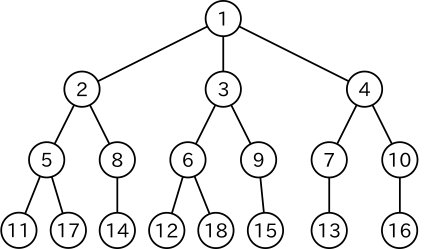
\includegraphics[width=.45\linewidth]
                      {initial-spanning-tree-18-example.pdf}
    }
    \caption{全域木の例}
    \label{fig:initial-spanning-tree-example}
  \end{figure}
\end{example}

\section{実験}
\label{sect:exp-reduce-by-initial}

\section{結果}
\label{sect:result-reduce-by-initial}

%
\chapter{枝刈りによる探索空間の削減}
\label{chap:reduce-by-prune}
枝刈りによって探索空間を削減する.
本稿では,直径の下界を計算し,定理\ref{thm:gmg-geometric-property}
の条件\ref{gmg-geom-b}を満足するか求めることで実現する.

\section{直径の下界の計算}
\label{sect:distance-lower-bound}
直径の下界を計算する方法を与える.まず,次のグラフを定義する.
\begin{definition}
  探索途中のグラフ$G$が与えられ,$i$番目の辺$e_i\in E$の追加判定および追加が
  行われたとする.$G$の辺と追加が未決定の辺すべて($\{e_j\}_{j>i}\subseteq E$)
  を合わせたグラフを\textbf{最大グラフ}と定義する.
  このとき,最大グラフのもとになったグラフを\textbf{最小グラフ}と呼ぶ.
\end{definition}
\begin{example}
  図\ref{fig:min-max-graph}に例を示す.最小グラフの破線部分は追加の
  判定が行われていない辺を表す.最大グラフは,最小グラフの追加未決定の辺を
  すべて追加したグラフとなっている.
\end{example}
\begin{figure}
  \centering
  \subfloat[最小グラフ]{
    \includegraphics[width=.4\linewidth]
                    {min-graph-example.pdf}
  }\hfill
  \subfloat[最大グラフ]{
    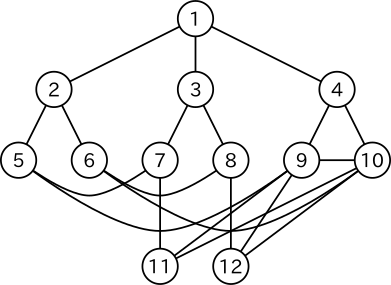
\includegraphics[width=.4\linewidth]
                    {max-graph-example.pdf}
  }
  \caption{最小グラフと最大グラフの例}
  \label{fig:min-max-graph}
\end{figure}

直径の下界は,最大グラフの直径を計算すればよい.もし直径の下界が
定理\ref{thm:gmg-geometric-property}の条件\ref{gmg-geom-b}を
満たさない場合,それはどのように辺を追加しても条件を満たさないので,
その場で探索を打ちきることができる.

\section{頂点間距離の高速な更新法}
\label{sect:faster-min-max}
第\ref{chap:basic-algorithm}章にて,グラフが枝刈りの対象となるかを
判定するには,追加する辺の頂点間距離と直径の下界を求める必要があることを述べた.
本節では,これらの値を高速に計算するため,辺の追加と削除に対して,頂点間距離と
直径の下界を更新するアルゴリズムを与える.
探索空間の削減にはつながらないが,計算量が削減され,実行時間の短縮が期待できる.
また,この方法は辺の追加と削除に対する媒介中心性の高速な計算法への応用が期待できる.

グラフ$G=(V,E),V=\{1,\ldots n\}$のすべての頂点の組$(s,t)$の距離$d(s,t)$と
距離が$d(s,t)$となる最短経路の数$\sigma(s,t)$が与えられているとする.
まず,追加と削除に共通するいくつかの補題を示す.
\begin{lemma-without-proof}[Brandes\cite{Brandes2001}]
  $G=(V,E)$の異なる2頂点$s,t\in V$に対して,$s$から$t$への最短経路
  $G_{st}=(V_{st},E{st})$が$i\in V$を含む,すなわち$i\in V_{st}$であるための
  必要十分条件は
  \[ d(s,t)=d(s,i)+d(i,t) \]
  が成り立つことである.
\end{lemma-without-proof}
\begin{lemma-without-proof}[難波ら\cite{Namba2016}]
  $G=(V,E)$の異なる2頂点$s,v\in V$と辺$\{i,j\}\in E$を考える.
  $s$から$t$への最短経路$G_{st}=(V_{st},E_{st})$が有向辺$(i,j)$を含む,
  すなわち$(i,j)\in E_{st}$が成り立つための必要十分条件は
  \[ d(s,t)=d(s,i)+d(j,t)+1 \]
  が成り立つことである.
\end{lemma-without-proof}
\begin{lemma-without-proof}[Brandes\cite{Brandes2001}]
  $G=(V,E)$の異なる2頂点$s,t\in V$に対して,$s$から$t$への最短経路の中で
  $i$を通るものの個数$\sigma_{st}(i)$は次式で与えられる.
  \[ \sigma(s,t)=\begin{aligned}\begin{cases}
    \sigma(s,i)\sigma(i,t) & d(s,t)=d(s,i)+d(i,t)\mathrm{のとき} \\
    0 & \mathrm{それ以外のとき}
  \end{cases}\end{aligned} \]
\end{lemma-without-proof}

次の補題は,ある2頂点間の最短経路の個数と,その経路に含まれる
短い最短経路の個数との関係を示す.
\begin{lemma}
  \label{lemma:number-of-paths}
  $d(s,t)=d(s,v)+d(v,t)$である$v\in V$(ただし$v\neq s,v\neq t$)について,
  \begin{equation}
    \label{eq:number-of-paths}
    \sigma(s,t)=\left(
    \sum_{v}\sigma(s,v)\sigma(v,t)\right) / (d(s,t)-1)
  \end{equation}
  が成り立つ.
\end{lemma}
\begin{proof}
  $s$と$t$の間の一般的な経路を図\ref{fig:proof-number-of-paths}に示す.
  \begin{figure}
    \centering
    \def\svgwidth{.5\columnwidth}
    \input{proof-number-of-paths.pdf_tex}
    \caption{$s$と$t$の一般的な最短経路}
    \label{fig:proof-number-of-paths}
  \end{figure}
  $s$からの距離が一定の頂点を並べて,一つの層とする.$d(s,v)=k$なる頂点
  $v$の集合を,第$k$層と定義し,$L_k$と表す.
  $L_k$に属する頂点の数を$n_k$,$l$番目の頂点を$v_{kl}$と表す.
  ここで,すべての層に属する頂点$v$は,隣接する層以外の層に属する頂点$w$と
  隣接しないことに注意する.もしそのような頂点が存在すると,最短経路長が
  変化する.式\ref{eq:number-of-paths}の両辺に$d(s,t)-1$を掛けて,
  \begin{equation}
    \sigma(s,t)(d(s,t)-1)=\sum_{v}\sigma(s,v)\sigma(v,t)
    \label{eq:number-of-paths1}
  \end{equation}
  となる.式\ref{eq:number-of-paths1}の右辺を,
  図\ref{fig:proof-number-of-paths}にならって変形して,
  \begin{equation}
    \sum_{v}\sigma(s,v)\sigma(v,t)=
    \sum_{k=1}^m\sum_{l=1}^{n_k}\sigma(s,v_{kl})\sigma(v_{kl},t)
    \label{eq:number-of-paths2}
  \end{equation}
  とする.二つの頂点$v$と$w$について,
  \begin{align*}
    a(v,w)=
    \begin{cases}
      1 & vとwが隣接しているとき \\
      0 & vとwが隣接していないとき
    \end{cases}
  \end{align*}
  と定義する.
  各々の$\sigma(s,v_{kl})\sigma(v_{kl},t)$について議論する.
  定義に沿って式を変形すると,
  \begin{align}
    &\sigma(s,v_{kl})\sigma(v_{kl},t)\nonumber\\
    =&\left(\sum_{v'\in L_{k-1}}\sigma(s,v')a(v',v_{kl})\right)
    \left(\sum_{v'\in L_{k+1}}\sigma(v_{kl},v')a(v',t)\right)
    \nonumber\\
    =&\left(\sum_{v''\in L_{k-2}}\sum_{v'\in L_{k-1}}
    \sigma(s,v'')a(v'',v')a(v',v_{kl})\right)
    \left(\sum_{v'\in L_{k+1}}\sum_{v''\in L_{k+2}}
    a(v_{kl},v')a(v',v'')\sigma(v'',t)\right)
    \nonumber\\
    &\vdots\nonumber\\
    =&\left(\sum_{(v_1,\ldots,v_{k-1})\in L_1\times\cdots\times L_{k-1}}
    a(s,v_1)\cdots a(v_{k-1},v_{kl})\right)
    \left(\sum_{(v_{k+1},\ldots,v_m)\in L_{k+1}\times\cdots\times L_m}
    a(v_{kl},v_{k+1})\cdots a(v_m,v_t)\right)\nonumber\\
    =&\sum_{
      (v_1,\ldots,v_{k-1},v_{k+1},\ldots,v_m)\in
      L_1\times\cdots\times L_{k-1}\times L_{k+1}\times\cdots\times L_m
    }
    a(s,v_1)\cdots a(v_{k-1},v_{kl})a(v_{kl},v_{k+1})\cdots a(v_m,t)
    \label{eq:number-of-paths3}
  \end{align}
  となる.式\ref{eq:number-of-paths3}を式\ref{eq:number-of-paths2}に
  代入すると,
  \begin{align}
    &\sum_{k=1}^m\sum_{l=1}^{n_k}\sigma(s,v_{kl})\sigma(v_{kl},t)\nonumber\\
    =&\sum_{k=1}^m\sum_{l=1}^{n_k}\sum_{
      (v_1,\ldots,v_{k-1},v_{k+1},\ldots,v_m)\in
      L_1\times\cdots\times L_{k-1}\times L_{k+1}\times\cdots\times L_m
    }
    a(s,v_1)\cdots a(v_{k-1},v_{kl})a(v_{kl},v_{k+1})\cdots a(v_m,t)\nonumber\\
    =&\sum_{k=1}^m\sum_{(v_1,\ldots,v_m)\in L_1\times\cdots\times L_m}
    a(s,v_1)\cdots a(v_m,t)\nonumber\\
    =&m\left(\sum_{(v_1,\ldots,v_m)\in L_1\times\cdots\times L_m}
    a(s,v_1)\cdots a(v_m,t)\right)
    \label{eq:number-of-paths4}
  \end{align}
  とできる.式\ref{eq:number-of-paths4}の総和の対象が$1$となるのは,
  $a(s,v_1),\ldots,a(v_m,t)$のすべてが$1$のとき,
  すなわち,$s$と$t$の最短経路となっているときである.
  従って,総和の値は$s$と$t$の最短経路の数を一致し,
  式\ref{eq:number-of-paths4}は$m\sigma(s,t)$と等しい.
\end{proof}

\subsection{辺の追加に対する頂点間距離の更新}
\label{subsect:update-path-length}
$G$に辺$e=\{\alpha,\beta\}\notin E(G)$を追加したた後の頂点間距離$d'(s,t)$と
最短経路数$\sigma'(s,t)$を求める.
一般性を失うことなく,$s<t,\,d(s,\alpha)\leq d(s,\beta)$とできる.

アルゴリズムをアルゴリズム\ref{algo:update-distance-on-insert}に示す.
\begin{algorithm}
  \caption{辺$\{\alpha,\beta\}$が追加されたときの$d'(s,t)$と$\sigma'(s,t)$の
  計算}\label{algo:update-distance-on-insert}
  \begin{algorithmic}[1]
    \Require $G=(V,E),\,d(s,t),\,\sigma(s,t)$
    \Ensure $d'(s,t),\,\sigma'(s,t)$
    \State $d'$と$\sigma'$の初期値を$d$と$\sigma$の値にしておく
    \ForAll{$(s,t)\in V\times V,\,s<t$}
    \State $(\alpha,\beta)$のうち$s$に近いほうを$\alpha$とする
    \If{$d(s,\alpha)<d(s,\beta)$かつ$d(s,t)>d(s,\alpha)+d(\beta,t)+1$}
    \State $d'(s,t)\gets d(s,\alpha)+d(\beta,t)+1$
    \State $d'(t,s)\gets d(s,\alpha)+d(\beta,t)+1$
    \State $\sigma'(s,t)\gets \sigma(s,\alpha)\sigma(\beta,t)$
    \State $\sigma'(t,s)\gets \sigma(s,\alpha)\sigma(\beta,t)$
    \ElsIf{$d(s,\alpha)<d(s,\beta)$かつ$d(s,t)=d(s,\alpha)+d(\beta,t)+1$}
    \State $\sigma'(s,t)\gets \sigma(s,t)+\sigma(s,\alpha)\sigma(\beta,t)$
    \State $\sigma'(t,s)\gets \sigma(s,t)+\sigma(s,\alpha)\sigma(\beta,t)$
    \Else
    \EndIf
    \EndFor
  \end{algorithmic}
\end{algorithm}

\subsection{辺の削除に対する頂点間距離の更新}
\label{subsect:update-lower-bound-of-diameter}
$G$から辺$e=\{\alpha,\beta\}\in E(G)$を削除した後の頂点間距離$d'(s,t)$と
最短経路数$\sigma'(s,t)$を求める.
一般性を失うことなく,$s<t,\,d(s,\alpha)\leq d(s,\beta)$とできる.

削除による影響を受けない場合は,$\cdots$である.
削除により,頂点間距離が変化せず,経路の個数が変化する場合は,$\cdots$である.
削除により,頂点間距離が変化する場合は,$\cdots$である.

次に,頂点間距離の更新が行われる組$(s,t)$の$\sigma'(s,t)$について議論する.
まず,準備のため次を示す.
\begin{collary}
  $\sigma'(s,t)$を再計算するには,すべての$d'(s,t)>d'(u,v)$の$\sigma'(u,v)$
  を先に計算しなければならない.
\end{collary}
\begin{proof}
  補題\ref{lemma:number-of-paths}の式\ref{eq:number-of-paths2}を見ると,
  $s$と$t$の最短経路の中に$d'(s,t)>d'(u,v)$なる$u$と$v$の最短経路が含まれ,
  そのような$u,v$に対する$\sigma'(u,v)$が含まれる.
\end{proof}
更新の対象となる頂点組の列$\{(s_i,t_i)\}$を更新後の距離$d'$の昇順に,
定理\ref{lemma:number-of-paths}の式を用いて,$\sigma'(u,v)$を求める.

アルゴリズムをアルゴリズム\ref{algo:update-distance-on-remove}に示す.
\begin{algorithm}
  \caption{辺$\{\alpha,\beta\}$が削除されたときの$d'(s,t)$と$\sigma'(s,t)$の
  計算}\label{algo:update-distance-on-remove}
  \begin{algorithmic}[1]
    \Require $G=(V,E),\,d(s,t),\,\sigma(s,t)$
    \Ensure $d'(s,t),\,\sigma'(s,t)$
    \State $d'$と$\sigma'$の初期値を$d$と$\sigma$の値にしておく
    \State $P\gets\varnothing$
    \Comment{更新の対象となる頂点組$(s,t)$}
    \ForAll{$(s,t)\in V\times V,\,s<t$}
    \State $\textrm{npath}\gets$\Call{Path num not contain}{$s,t$}
    \If{$d(s,t)=\infty$または$\textrm{npath}>0$}
    \State $\sigma'(s,t)\gets\textrm{npath},\:\sigma'(t,s)\gets\textrm{npath}$
    \Else\Comment{削除により頂点間距離が変化する}
    \State $d_{\min}\gets \infty$
    \ForAll{$v\in V$}
    \If{\Call{Path num not contain}{$s,v$}$>0$かつ
      \Call{Path num not contain}{$v,t$}$>0$}
    \State $d_{\min}\gets\min\left(d_{\min},d(s,v)+d(v,t)\right)$
    \EndIf
    \EndFor
    \If{$d_{\min}=\infty$}
    \Comment{削除により連結でなくなった}
    \State $d'(s,t)\gets\infty,\:d'(t,s)\gets\infty$
    \State $\sigma'(s,t)\gets 0,\:\sigma'(t,s)\gets 0$
    \Else
    \State $d'(s,t)\gets d_{\min},\:d'(t,s)\gets d_{\min}$
    \State \parbox[t]{\linewidth}{
      $P\gets \{\ldots,(s_i,t_i),(s,t),(s_{i+1},t_{i+1}),\ldots\}$\\
      ただし,$d'(s_i,t_i)\leq d'(s,t)\leq d'(s_{i+1},t_{i+1}),\:$
      $(s_1,t_1),\ldots,(s_i,t_i),\ldots\in P$
    }
    \EndIf
    \EndIf
    \EndFor
    \ForAll{$i=\{1,\ldots,|P|\}$}\Comment{最短経路数を更新}
    \State $(s_i,t_i)\gets P_i$
    \State \parbox[t]{\linewidth}{
      $\sigma'(s_i,t_i)\gets$
      $\left(\sum_{v}\sigma(s_i,v)\sigma(v,t_i)\right) / (d'(s_i,t_i)-1)$ \\
      ただし,
      $v\in V,\,d'(s_i,t_i)=d'(s_i,v_i)+d'(v_i,t_i),\,v\neq s_i,\,v\neq t_i$
    }
    \EndFor
    \Procedure{Path num not contain}{$s,t$}
    \State $(\alpha,\beta)$のうち$s$に近いほうを$\alpha$とする
    \If{$d(s,t)<d(s,\alpha)+d(\beta,t)+1$}
    \State \textbf{return} $\sigma(s,t)$
    \Else
    \State \textbf{return} $\sigma(s,t)-\sigma(s,\alpha)\sigma(\beta,t)$
    \EndIf
    \EndProcedure
  \end{algorithmic}
\end{algorithm}

\section{実験}

\section{結果}
次数が3のときの実験結果を示す.
探索開始から最初の一般化ムーアグラフの発見における探索時間と状態の
取り出し回数を図\ref{fig:sinitr-time}と図\ref{fig:sinitr-node}に
それぞれ示す.また,一般化ムーアグラフの列挙におけるグラフ数と列挙時間と
状態の取り出し回数を図\ref{fig:sinitr-full-graph}と図\ref{fig:sinitr-full-time}と
図\ref{fig:sinitr-full-node}にそれぞれ示す.結果から,次のことが考察される.
指数関数的に増える(適当).

\begin{figure}
  \centering
  \includegraphics{the-sinitr-time.pdf}
  \caption{最初の一般化ムーアグラフの発見までの時間}
  \label{fig:sinitr-time}
\end{figure}
\begin{figure}
  \centering
  \includegraphics{the-sinitr-node.pdf}
  \caption{最初の一般化ムーアグラフの発見までの展開状態数}
  \label{fig:sinitr-node}
\end{figure}

\begin{figure}
  \centering
  \includegraphics{the-sinitr-full-graph.pdf}
  \caption{列挙された一般化ムーアグラフの数}
  \label{fig:sinitr-full-graph}
\end{figure}
\begin{figure}
  \centering
  \includegraphics{the-sinitr-full-time.pdf}
  \caption{一般化ムーアグラフの列挙に要した時間}
  \label{fig:sinitr-full-time}
\end{figure}
\begin{figure}
  \centering
  \includegraphics{the-sinitr-full-node.pdf}
  \caption{一般化ムーアグラフの列挙における展開状態数}
  \label{fig:sinitr-full-node}
\end{figure}

%
\chapter{一般化ムーアグラフの列挙}
本章では,第\ref{chap:reduce-by-initial-graph}章で導入した初期グラフの
妥当性(予想\ref{conj:gmg-cycle}と予想\ref{conj:spanning-tree})を検証する.
そのために,一般化ムーアグラフを重複なく列挙する方法を与え,実験を行う.

\section{列挙アルゴリズム}
\label{sect:enum-algorithm}
一般化ムーアグラフを重複なく列挙する,つまり,非同型なグラフを列挙する
方法を与える.そのためのアルゴリズムをアルゴリズム\ref{algo:gmg-enumeration}
に示す.ここで,$\text{Aut}(G)$をグラフ$G$の同型グラフの集合とする.

\begin{algorithm}[H]
  \caption{一般化ムーアグラフの列挙アルゴリズム}
  \label{algo:gmg-enumeration}
  \begin{algorithmic}[1]
    \Require $n,k$
    \Ensure 互いに非同型な$M(n,k)$の集合
    \Procedure{EnumerateGeneralizedMooreGraph}{}
    \State $G_I\gets\text{初期グラフ}$
    \State $\{e_i\}_{i\in\mathbb{N}}^M\gets G_I\text{の候補辺}$
    \State $Gs_1\gets\{G_I\}$
    \ForAll{$i\in\{1,\ldots,M\}$}
    \State $Gs_{i+1}\gets\varnothing$
    \ForAll{$G\in Gs_i$}
    \ForAll{$operator\in\{\text{追加オペレータ},\text{無追加オペレータ}\}$}
    \If{$G,e_i$に$operator$が適応でき,かつ,
      $operator(G,e_i)\notin\cup_{H\in Gs_{i+1}}\text{Aut}(H)$}
    \State $Gs_{i+1}\gets Gs_{i+1}\cup\{operator(G,e_i)\}$
    \EndIf
    \EndFor
    \EndFor
    \EndFor
    \State \textbf{return} $\{G\,|\,G\in Gs_{M+1},$
    $G\text{が正則で定理\ref{thm:gmg-geometric-property}を満たす}\}$
    \EndProcedure
  \end{algorithmic}
\end{algorithm}

\section{実験}
節\ref{sect:enum-algorithm}で定義したアルゴリズムを用いて,一般化ムーアグラフを
列挙し,第\ref{chap:reduce-by-initial-graph}章で導入した初期グラフの妥当性を
検証する.具体的には,初期グラフを変更してアルゴリズムを開始し,得られた
一般化ムーアグラフの個数が同じかを確認する.
検証する頂点数$n$と次数$k$は,$k=3,4$と
\begin{equation*}
  \begin{aligned}
    n=\begin{cases}
      4,6,8,10,12,14,16,18 & (k=3) \\
      5,6,7,8,9,10,11 & (k=4)
    \end{cases}
  \end{aligned}
\end{equation*}
とする.実験を行った環境は,表\ref{tab:env-lab}の通りである.

\section{結果}
アルゴリズムにより得られた一般化ムーアグラフの数を表\ref{tab:ginitr-ngraph-iso}
に示す.

% latex table generated in R 3.4.2 by xtable 1.8-2 package
% Thu Jan  4 15:06:44 2018
\begin{table}[ht]
\centering
\caption{初期グラフを変更したときの互いに非同型な一般化ムーアグラフの数} 
\label{tab:ginitr-ngraph-iso}
\begin{tabular}{lrrr}
  \hline
$(n,d)$ & 基本初期グラフ & 閉路初期グラフ & 全域木初期グラフ \\ 
  \hline
(4,3) &   1 &   1 &   1 \\ 
  (6,3) &   2 &   2 &   2 \\ 
  (8,3) &   2 &   2 &   2 \\ 
  (10,3) &   1 &   1 &   1 \\ 
  (12,3) &   2 &   2 &   2 \\ 
  (14,3) &   7 &   7 &   7 \\ 
  (16,3) &   6 &   6 &   6 \\ 
  (18,3) &   1 &   1 &   1 \\ 
  (5,4) &   1 &   1 &   1 \\ 
  (6,4) &   1 &   1 &   1 \\ 
  (7,4) &   2 &   2 &   2 \\ 
  (8,4) &   6 &   6 &   6 \\ 
  (9,4) &  16 &  16 &  16 \\ 
  (10,4) &  24 &  24 &  24 \\ 
  (11,4) &  37 &  37 &  37 \\ 
   \hline
\end{tabular}
\end{table}


結果のとおり,初期グラフを変更したことによって列挙されない一般化ムーアグラフは
存在しないことが分かる.つまり,実験を行った頂点数と次数の範囲では,
初期グラフの変更は妥当である.


\chapter{結論}
本論文では,全探索法を基にした一般化ムーアグラフの探索の高速化および高効率化に
ついて述べた.まず,一般化ムーアグラフを定義して,その性質を示し証明を与えた.
次に,この性質を利用して,一般化ムーアグラフを探索するアルゴリズムを定めた.
最後に,探索空間の削減による高効率化の方法を与え,その効果を実験によって示した.

本論文では,高効率化の方法として,探索の初期状態を変更することと
枝刈りの二つを提案した.
探索の初期状態の変更とは,初期状態のグラフに予めいくつかの辺を追加した状態を
新たな初期状態とすることである.本論文では,辺を二本追加して閉路を含むようにした
グラフと,全域木の二種類を提案した.実験の結果から,一般的な場合では全域木から
探索を始める場合が最も効率が良いことが分かった.また,閉路を含むグラフは
ある頂点数と次数の組合せにおいて,効率が悪くなることが示された.
また,枝刈りの方法として,探索途中のグラフの直径の下界を用いる方法を提案した.
枝刈りによって探索空間が削減され高効率化は達成されたが,
頂点数および次数が小さい場合に探索に時間がかかることが結果から示された.

今後の課題は,提案した方法を用いて一般化ムーアグラフの存在を調べることや,
提案した初期状態から探索を開始することの妥当性の証明,
および,一般化ムーアグラフが存在しない時の,平均頂点間距離最小の正則グラフの
研究である.


\chapter*{謝辞}
本論文は筆者が岡山大学工学部情報系学科に在籍中の研究結果をまとめたものである.
本研究を行うにあたり,ご指導を頂いた岡山大学大学院自然科学研究科産業創成工学専攻
高橋規一教授に深謝の意を表する.
また,情報数理工学研究室の皆様には,日常の議論を通して多くの知識や示唆を頂いた.
ここに謝意を表する.

\appendix

\chapter{実験プログラム}
\label{chap:program}

\chapter{一般化ムーアグラフのリスト}



\bibliography{../res/MyCollection}

\end{document}
